\documentclass[12pt,oneside,a4paper]{report}
%-------------------------------------------------------
% PACKAGES

\usepackage{float}
\usepackage{natbib}
\usepackage{booktabs}
\usepackage{multirow}
\usepackage{amsmath}
\usepackage{graphicx}
\usepackage{bm}
\usepackage[toc,page]{appendix}
\usepackage{graphicx}
\usepackage{subcaption}
\usepackage[colorlinks=true,linkcolor=blue, citecolor=blue]{hyperref}

% COMANDS FOR TABLE
\usepackage{dcolumn}
\usepackage{caption}
\newcommand\fnote[1]{\captionsetup{font=scriptsize, format=hang}\caption*{#1}}


% Econometrics notations
\newcommand{\cov}{\operatorname{cov}}
\newcommand{\var}{\operatorname{var}}
\newcommand{\mX}{\bm X}
\newcommand{\vx}{\bm x}
\newcommand{\vbeta}{\bm \beta}
\newcommand{\dto}{\stackrel{d}{\longrightarrow}}

%-------------------------------------------------------
% CONFIG

\graphicspath{{./figs/}}


%-------------------------------------------------------
% PRE-TEXT CONTENT

\title{Assessing Fiscal Distress in Subnational Governments: The Case of Brazil}
\author{Francisco Alves}
\date{2017}

%-------------------------------------------------------
% TEXT BODY CONTENT

\begin{document}

\begin{titlepage}
    \centering
    {\scshape\LARGE University of York\par}
    \vspace{1cm}
    {\scshape\Large Department of Economics and Related Studies\par}
    \vspace{1.5cm}
    {\huge\bfseries Assessing Fiscal Distress in Subnational Governments: The Case of Brazil\par}
    \vspace{2cm}
    {\Large\itshape Francisco Alves\par}
    {MSc Economics and Public Policy\par}
    \vfill
    supervised by\par
    Dr.~Michal \textsc{Horvath}

    \vfill

% Bottom of the page
    {\large \today\par}
\end{titlepage}

% \begin{abstract}
% My abstract
% \end{abstract}

\tableofcontents

\chapter{Introduction} % 1000 words
\chapter{Literature Review}
\label{sec:literature-review}

As noted by \citet{baldacci2011b}, the literature that aims to build models that can provide early warning signals of fiscal sustainability problems tend to differ with respect to three major characteristics: the definition of the crisis event; the statistical methodology employed; and the set of explanatory variables used. Broadly following this differences, in section \ref{sec:fiscal-distress} we review theoretical definitions of fiscal sustainability in order to propose a definition of fiscal distress\footnote{For the purposes of this study, fiscal distress, fiscal stress, fiscal crisis, and debt crisis will be used as synonymous} event that will be used in this study. In section \ref{sec:ews} we present a general formulation of the early warning system problem and the methodological approach pursued in this study. Regarding the set of explanatory variables, since the main objective of this study is to assess the significance of the fiscal indicators used by the National Treasury Secretariat in their mandate to evaluate the payment capacity of subnational governments, the explanatory variables are already defined. Therefore we let the presentation of the fiscal indicators for section \ref{sec:data} coupled with the exploratory analysis of the data.

% in section \ref{sec:brazil} we provide a brief overview of the evolution of fiscal distress events of SGNs that happened in the Brazilian economy since the 80s and 90s and the reforms initiatives that followed in order to characterize the present rules regarding borrowing by SGNs.

% \footnote{Although not used as much in the economic literature, early warning signals models are also called predictive models in the statistical and machine learning literature. The important difference is that there is no preoccupation with causal inference in this type of exercise}

\section{Fiscal Distress}
\label{sec:fiscal-distress}

The focus of this study will be on the empirical analysis of the main determinants of fiscal distress episodes in subnational governments in Brazil in the 2008-2016 period. Nevertheless, it is important a brief theoretical review of the most used concepts of fiscal sustainability so that an appropriate characterization of what fiscal distress event entails, or, and perhaps even more importantly, what it do not entail.

There are a few distinct ways in which fiscal sustainability is defined in the economic literature. Although they all in some way or another alludes to the more general concept of sustainability, understood here as a process that ``meets the needs of the present without compromising the ability of future generations to meet their own needs'' \citep{un1987}, the differences are important for the interpretation of the empirical results and should be emphasized at the outset.

A more narrow definition of fiscal sustainability equates it to solvency, that is, the ability of an entity, in the case of this study a subnational government, to make payments in order to service its debt obligations on the due date. Although certainly useful for corporations, this definition is far too stringent when applied to governments. The reasoning is not as much because governments do not actually default on its debt, but, as pointed out by \citet{burnside2005}, when it is clear that a policy mix is unsustainable, governments tend to take remedial actions in order to avoid an outright default. A more useful definition of fiscal sustainability takes this into account and can be equated ``to a government’s ability to indefinitely maintain the same set of policies while remaining solvent'' \citep[pg.11]{burnside2005}. Therefore it makes sense to speak of an unsustainable policy mix even though a default on the debt never actually took place. For the purposes of this study, both an explicit default on the debt and an unsustainable policy mix should be considered an indicator of a fiscal distress event. 

It is worth pointing out that in the definitions given so far, no distinction was made between solvency and liquidity problems. A country may believe itself to be solvent, but it still faces problems in meeting its obligations because of cash flows problems. The reason we don't pursue this distinction is less based on the fact that there are no theoretical differences between the two concepts, but because the empirical consequences of both difficulties are likely to be observationally equivalent \citep[pg.89]{chuhan2005}. Both solvency and liquidity are related to an entity ability to pay. However, especially because of the absence of clearly defined rules for bankruptcy in the public sector, the government willingness to pay also becomes important, in a tradition that goes back at least to \citet{eaton1981}. Again, however, for the purposes of this study, both are fiscal crisis episodes stemming from ability or willingness to pay are likely to be observationally equivalent.

One of the uses of fiscal sustainability that will not be used in this study is related to the costs, in terms of economic efficiency or growth, related to a given combination of fiscal and monetary policy. Although this use is suggested by \citet{burnside2005}, we shall make no claim in this study related to it.

After looking at the theoretical definitions of fiscal sustainability, its worth to take a closer look into how previous literature on EWS defined the debt crisis episodes for sovereign governments. \citet{manasse2003} defines a country to be in a debt crisis if either the government fails to meet principal or interest payment on external obligation on the due date as classified by Standard \& Poor's or if it receives a nonconcessional IMF loan in excess of 100 percent of its quota. \citet{fuertes2007} considers a country to be in default in a given year if the arrears increase over a threshold percentage of external debt and a rescheduling agreement is reached in which the amount of debt rescheduled exceeds the decrease in the arrears stock. \citet{baldacci2011b} uses a more general definition and considers a fiscal crisis not only the episodes of debt default or restructuring and recourse to exceptional financing, but also an implicit default crystallized in high inflation rates and a deterioration in market access measured by high bond yields pressures (where high is those that yield spreads that are more than two standard deviations away from the mean).

Although the empirical literature is of limited applicability in giving operational guidance in defining fiscal crisis episodes for this study because of differences in sovereign and subnational governments, it is possible to see that the theoretical elements discussed of solvency and liquidity are present. 

\section{Early Warning Systems}
\label{sec:ews}

Before we delve into the different methodological approaches used in the literature in early warning systems, we need a general framework to capture the purpose of an EWS model. Following \citet{fuertes2007}, we denote by $d_{it}$ the dummy variable that equals 1 if the state $i$ had a crisis event in period $t$ and 0 otherwise. Since the objective is to signal crisis in advance, the dependent variable $y_{it}$ of interest is forward-looking in nature, and it takes the value of one if a crisis happens during an $h$ time horizon, that is
\begin{equation}
y_{it} = \begin{cases} 
      1 & \text{if } d_{i,t+k} = 1 \text{ for any } k = 0, \dots, h-1\\
      0 & \text{otherwise}
   \end{cases}
\end{equation}

However, it is important to remark that the information set\footnote{The information set, usually denoted by $\Omega_t$ consists of the set of all potential explanatory variables that could be included in a regression model.} for predicting $y_{it}$ is that available at time $t-1$. To fix ideas, let the explanatory variable be the primary balance as a ratio of GDP and let $t = 2016$. A prediction $\hat{y}_{it} = 1$ from an EWS with horizon $h = 1$ implies that using the primary balance as a ratio to GDP from 2015 backwards, the model is signalling a potential crisis in 2016 for state $i$. Similarly, if $h = 2$, the model is signalling a potential crisis in 2016 or 2017. Note that again only the primary balance as a ratio to GDP from 2015 backward is used to make this prediction. 

In a more general notation, if we let $\vx$ denote the explanatory variables included in the model, and the past of $\vx$ for state $i$ as $\mX_{i,t-1} = \{\vx_{i,t-1}, \vx_{i,t-2}, \dots \}$, the prediction problem of an EWS with a given horizon $h$ is given by
\begin{equation}
\label{eq:classifier}
y_{it} = f(\mX_{i,t-1})
\end{equation}

In practice using the whole past $\mX_{i,t-1}$ of the explanatory variables is not possible, and we will follow other studies using only the last period variables, that is, $\vx_{i, t-1}$. This is not problematic as long as there are stock variables that can capture the effects of flows from previous periods.

For estimating the function $f$ in (\ref{eq:classifier}),  there are two major approaches in the literature on early warning systems. The ``indicators'' or ``signaling'' approach and the multivariate regression analysis approach \citep[pg. 5]{baldacci2011b}. The first approach belongs to the class of non-parametric methods. Their essential characteristic is that they do not assume a specific functional form for $f$, and simply try to estimate a smooth relationship between the explanatory and dependent variables. The second approach belongs to the class of parametric methods. In this case, a specific functional form for $f$ is assumed, and, with this knowledge at hand, the relevant parameters are estimated\footnote{\citet{james2013} is a nice introduction and overview of statistical learning techniques, both parametric and non-parametric. \citet{hastie2009} is a more advanced and complete treatment.}. In this study, we will take the latter approach. More specifically, we will make use of a limited dependent variable model know as logit regression\footnote{The specific characteristics of the model employed are discussed in section \ref{sec:econometric-model}}. 

As noted by \citet{baldacci2011b}, the main reason for using the multivariate approach in this study is the easily available null hypothesis significance tests that can be conducted to assess the statistical significance of both individual variables and collection of variables. This allows for a clean way to attain one of the objectives of this study, that is, to compare and contrast the current and the newly set of fiscal indicators used by the National Treasury Secretariat to assess the payment capacity of SGNs in Brazil.

% can we do NHST in non-parametric tests?

% \section{Fiscal Indicators}
% \label{sec:fiscal-indicators}

 % This section aims not only to present the fiscal indicators, but also to take a step back and give a brief overview of the broader institutional context that characterizes the Brazilian fiscal framework and that culminated in the current legislation regarding subnational borrowing in Brazil. 

% - Brazil Subnational Debt Restructuring of the 1990s
% - Fiscal Responsibility Law
% - 2016 Debt Relief Plan for the States and the Federal District (PLP 257/2016, LC 156/2016)
% - 2017 Fiscal Recovery Regime for the States and the Federal District (PLC 39/2017, LC 159/2017)
% - Payment Capacity Evaluation Methodology

% Although the above characterization could be employed to describe the recent economic history of several countries, Brazil might as well be the canonical example. A federation with one Federal District, 26 states, and 5,570 municipalities, Brazil experienced in the 80s and 90s repeated fiscal crisis of subnational entities with three rounds of debt restructurings. These episodes severely threatened the success of several macroeconomic stabilization programs that hoped to control the three-to-four-digit annual inflation rates that wreak havoc the Brazilian economy from 1980 through 1994. It was only with the success of the Real Plan in fighting the hyperinflation, and with a more comprehensive debt restructuring that aimed to correct the underlying SNG fiscal problems, that the political and economic conditions enabled for a complete reformulation of the fiscal institutions in place, culminating with the publication of a Fiscal Responsibility Law (FRL) in 2000 \citep[p. 34-35]{manoel2013}. 

% The FRL was a comprehensive law that promoted several changes in the institutions related to the Brazilian budgetary process. However, for the purposes of this study, the focus will be on the controls that were put forth for SGNs borrowings. In Brazil, if the central government must offer a guarantee for an individual borrowing operation, then the Finance Ministry, through the National Treasury Secretariat (NTS), must assess that entity ``payment capacity'' before the operation is authorized. The current methodology employed by NTS was enacted in 2012 and makes use of several fiscal indicators to classify the SGNs entities in different credit classifications, similar in spirit to the process adopted by rating agencies in giving credit ratings. However, this methodology is currently being revised \footnote{The NTS published the new set fiscal indicators and opened the methodology for a public revision process in the period of 10/05/2017 to 30/06/2017. The material related to this revision is available at \url{http://www.tesouro.fazenda.gov.br/sistemagarantiauniao}}, as the NTS is looking for an alternative suite of fiscal indicators that are more transparent and more easily calculated. In this context, the assessement of the statistical and practical significance of both the current and the newly set of fiscal indicators used by the National Treasury Secretariat to assess the fiscal sustainability of subnational governments in Brazil is both necessary and timely. 
 % 2500 words
\chapter{Methods}
\label{sec:methods}

\section{Data}
\label{sec:data}

The majority of the explanatory variables used in this study are derived from the fiscal reports made available by the National Treasury Secretariat (NTS), who is responsible for collecting primary fiscal data from subnational governments in Brazil. The consolidated dataset is available at \url{https://github.com/fjuniorr/junior2017}. The focus of this section is to present an exploratory and descriptive analysis of the fiscal indicators that are used (or whose use is proposed in the new methodology) by the NTS in its payment capacity evaluation.

The final dataset used in this study consists of fiscal indicators compiled for the 26 states and the federal district from 2008 through 2016, totaling $n = 243$ observations. Since the explanatory variables will be lagged 1 year, the sample size is reduced from 2009-2016, totaling $n = 216$ for estimation purposes.

For the purposes of this study, the publication of a decree of financial calamity\footnote{\url{http://economia.estadao.com.br/noticias/geral,veja-por-que-os-estados-decretam-calamidade-financeira,10000096967}} will be the event that characterizes a fiscal crisis in a given state-year. The reasoning is that, consistent with the discussion made in section \ref{sec:fiscal-distress}, the decree of public calamity, although legally questionable\footnote{\url{http://g1.globo.com/bom-dia-brasil/noticia/2016/12/calamidade-financeira-de-estados-nao-e-reconhecida-pelo-governo.html}}, clearly signals that the policy mix has become unsustainable, and, even if there are still doubts about the states ability to pay in terms of solvency and liquidity, definitely they don't have the willingness to pay. Therefore the dummy default $d_{it}$ will take the value of one in 2016 for the states of Rio de Janeiro (RJ), Rio Grande do Sul (RS), and Minas Gerais (MG). Following previous studies, we will use the time-horizon of one year $h=1$, meaning that the forward-looking independent variable $y_{it}$ will be equal to $d_{it}$. 

Table \ref{tbl:desc_stats} presents descriptive statistics for the explanatory variables that will be used in this study. With respect to the fiscal indicators of the current methodology, four variables are especially different in the non-calamity/calamity dichotomy.  These variables show that the states that did not declared financial calamity have lower debt (Gross debt / Net current revenue - $0.86 \pm 0.56$ \textit{vs} $2.19 \pm 0.13$), a less expensive payroll cost (Compensation of employees / Net current revenue - $0.54 \pm 0.09$ \textit{vs} $0.74 \pm 0.04$), more savings (Current fiscal balance / Current revenue - $0.23 \pm 0.17$ \textit{vs} $0.00 \pm 0.12$) and more investments (Gross investment in nonfinancial assets / Total expenditure - $0.09 \pm 0.04$ \textit{vs} $0.03 \pm 0.01$) than those states that did declare financial calamity. The ratio Primary balance / Debt Service also shows that the calamity states were running on average a primary deficit ($-0.66 \pm 1.00$), although with too much variability overall to characterize the differences between the two groups. The same holds true for the ratio Social contributions / Social benefits that shows that the states that declared calamity on average have a larger social security deficit, although with large variability overall.

In regard to the fiscal indicators proposed by the new methodology, the non-calamity/calamity difference is startling. Besides the already identified higher debt and lower savings of calamity states, they have very large liquidity problems compared to the non-calamity states (Current liabilities / Cash and cash equivalents - $0.47 \pm 0.36$ \textit{vs} $2.57 \pm 0.70$). Although with the data available it is not possible to distinguish how big is the arrears stock, this proxy indicates that the number is likely to be very large for calamity states.

\begin{table}[!ht]
\centering
\caption{Descriptive statistics} \label{tbl:desc_stats}
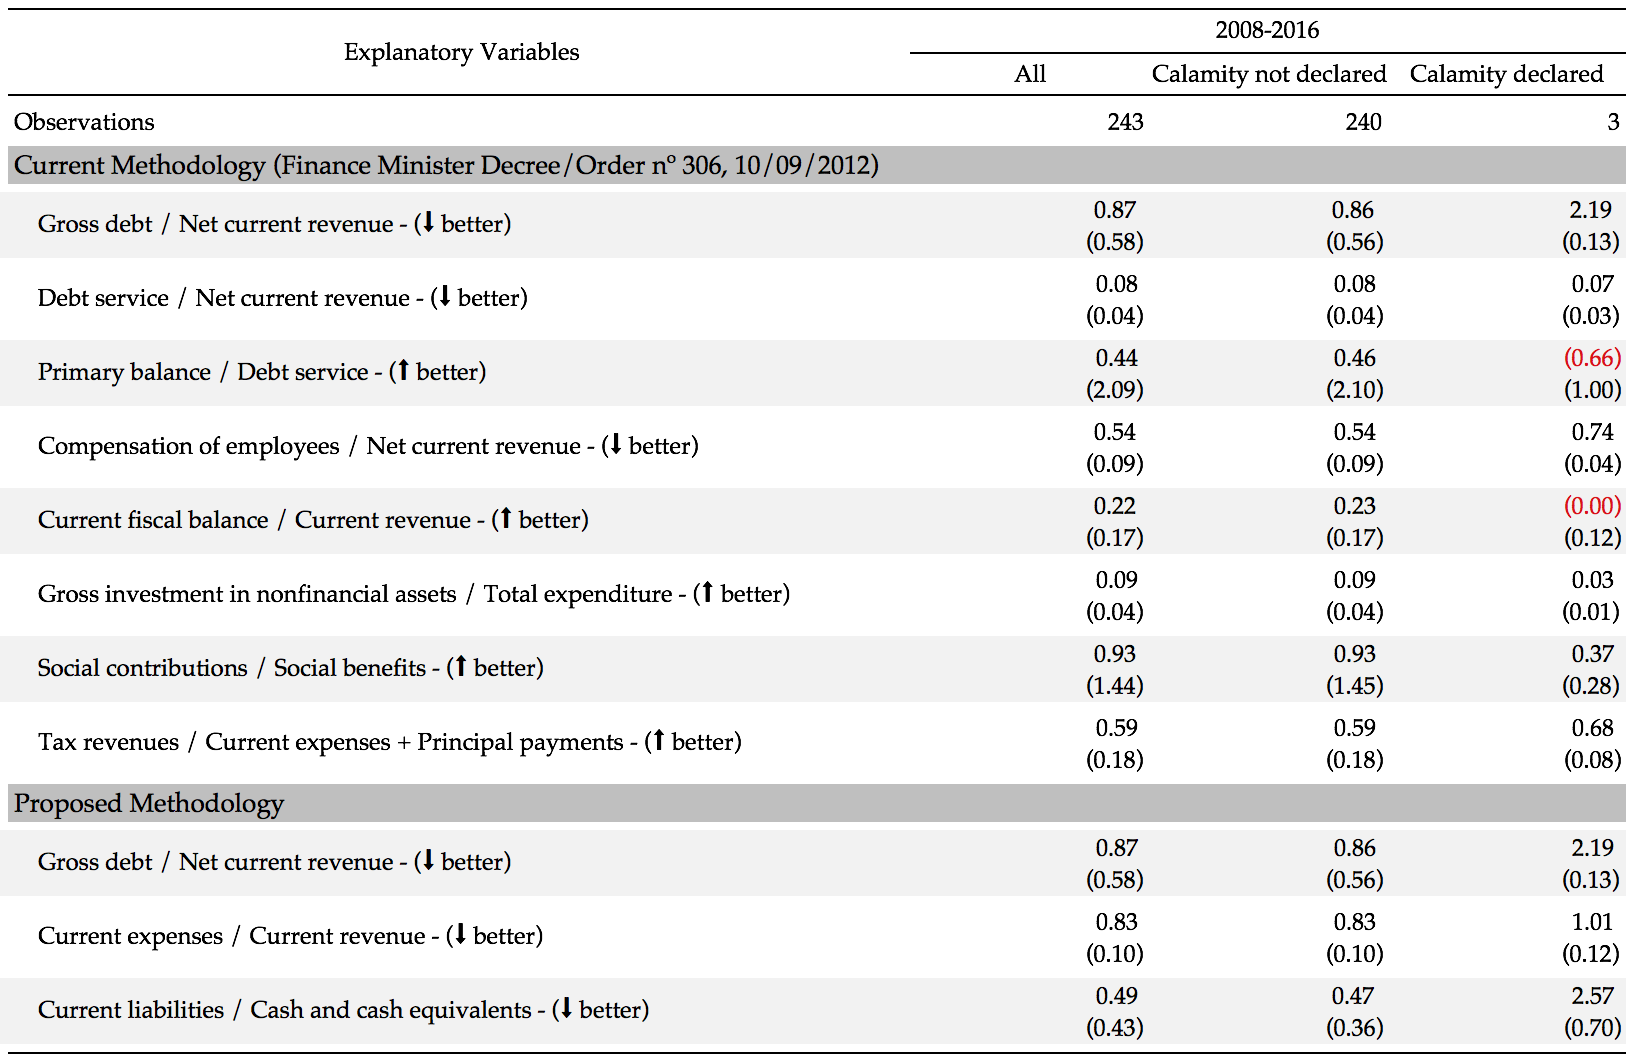
\includegraphics[scale=0.50]{tables/desc_stats.png}
\fnote{Notes: \\
       1) All variables are reported as averages across the observations with standard deviation reported in parentheses \\
       2) The variable Gross debt / Net current revenue is reported twice only to acknowledge that it was present in both methodologies. The variables Current fiscal balance / Current revenue and Current expenses / Current revenue have a different calculation rule, but convey the same information. For econometric purposes, only one will be used to avoid multicollinearity issues}
\end{table}

One particular feature of the data that is not possible to gauge from table \ref{tbl:desc_stats} is for how long the states that declared financial calamity in 2016 had worse fiscal indicators than the other states. Figure \ref{fig:evolution_capag} shows this evolution for the fiscal indicators of the new methodology. The major trend is that in the whole 2008-2016 the two groups of states were different, but, the states that declared financial calamity in 2016 had a major fiscal deterioration in 2015 and 2016. The evolution of Current liabilities / Cash and cash equivalents is particularly marked, going from an average of $0.98$ in 2014, to $1.88$ in 2015 and ballooning to $2.57$ in 2016.

\begin{figure}[!ht]
\centering
\begin{subfigure}{.5\textwidth}
  \centering
  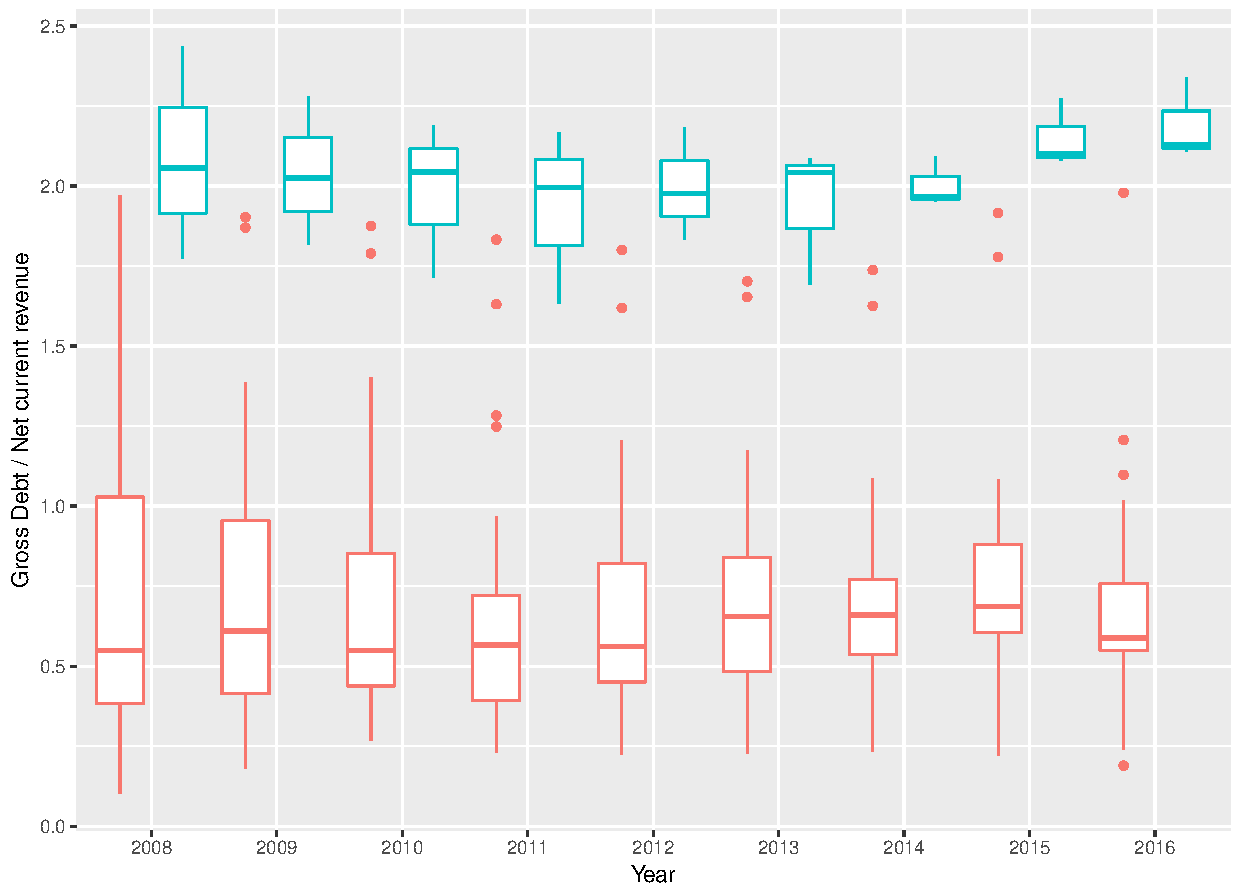
\includegraphics[width=\linewidth]{viz_capag_idc.pdf}
  \caption{Gross Debt / Net current revenue}
  \label{fig:capag_pc}
\end{subfigure}%
\begin{subfigure}{.5\textwidth}
  \centering
  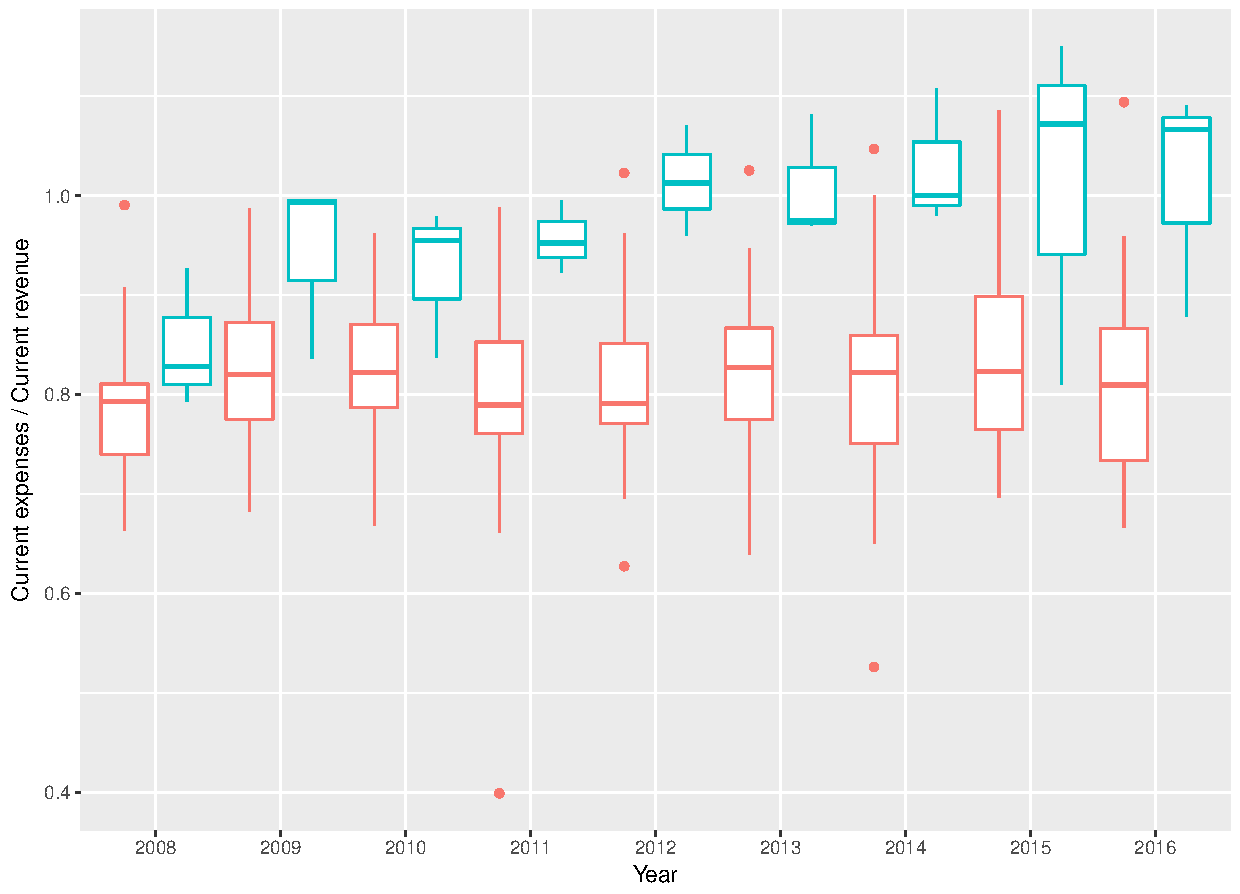
\includegraphics[width=\linewidth]{viz_capag_pc.pdf}
  \caption{Current expenses / Current revenue}
  \label{fig:capag_il}
\end{subfigure}

\begin{subfigure}{\textwidth}
  \centering
  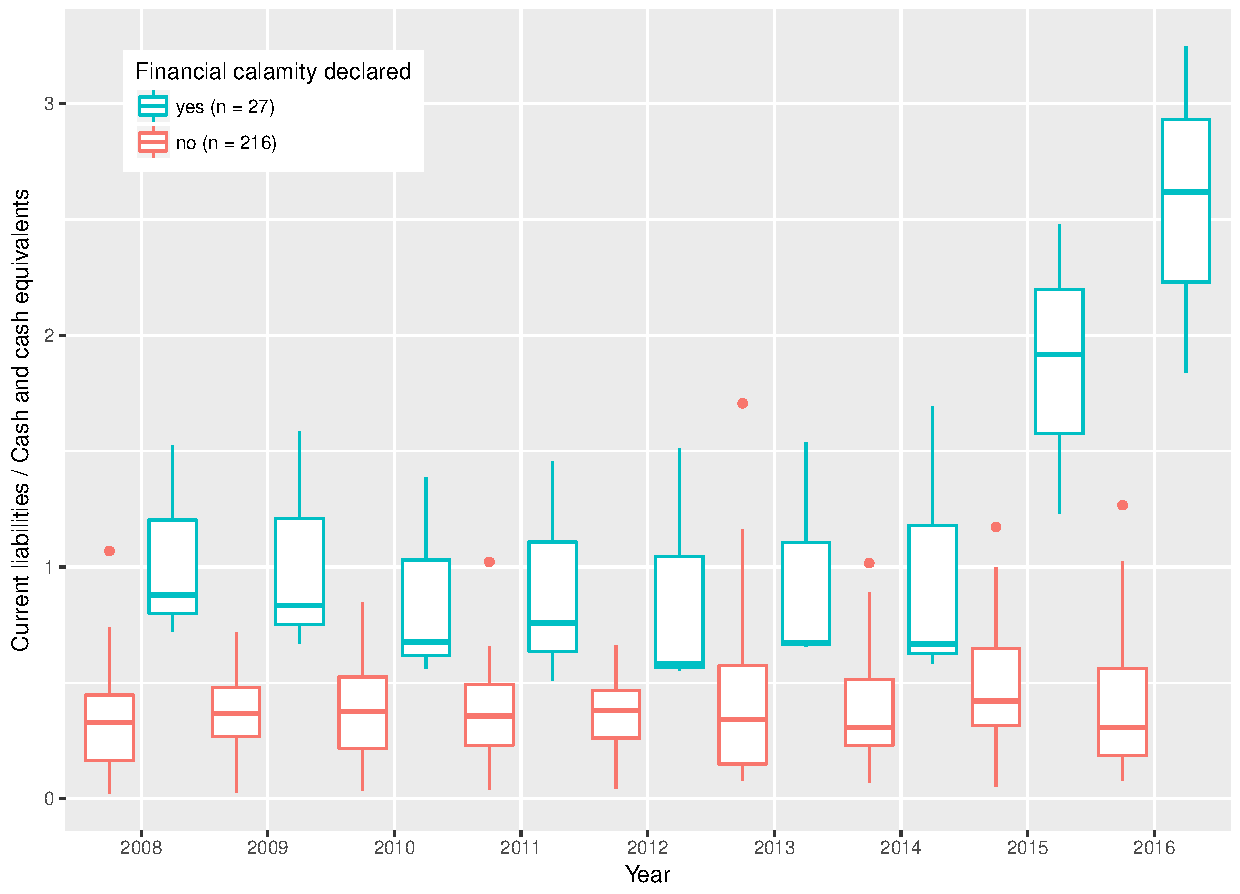
\includegraphics[width=\linewidth]{viz_capag_il.pdf}
  \caption{Current liabilities / Cash and cash equivalents}
  \label{fig:capag_idc}
\end{subfigure}%

\caption{Evolution of SGNs Financial Ratios proposed in the Payment Capacity Evaluation - 2008-2016}
\label{fig:evolution_capag}
\caption*{Source: Own elaboration}
\end{figure}

\clearpage

\section{Econometric Model}
\label{sec:econometric-model}

In this section we mostly follow the expositions and results from \citet{greene2011}, \citet{heij2004} and \citet{davidson2004} adapted to the notation used in this study. 

To assess the relative importance of these several potential explanatory variables, we need to use multiple regression analysis. The main model in this study will be a logit model, which is a special case of a binary response model. The binary response model can be derived from an underlying latent variable model. The latent variable model is
\begin{equation}
y^*_{it} = \vx'_{i,t-1}\vbeta + \epsilon_{it}, \quad (i = 1, \dots, N \text{ and } t = 1, \dots, T)
\end{equation}

This is the so-called index function, $\vx_{i,t-1}'\vbeta$ is the systematic term and $\epsilon_{it}$ is an idiosyncratic error term. In our case, the latent variable $y^*_{it}$ can be interpreted as either a propensity to default or as a measure of creditworthiness. We don't observe $y^*_{it}$, only $y_{it}$ according to
\begin{equation}
y_{it} = \begin{cases} 
      1, & \text{if } y^*_{it} \geq 0 \\
      0, & \text{if } y^*_{it} < 0 
   \end{cases}
\end{equation}
Assuming that $\epsilon_{it}$ has a standard logistic distribution we have that
\begin{align}
\label{eq:model}
\begin{split}
\Pr(y_{it} = 1 \mid \vx_{i,t-1}) &= \Pr(y^*_i \geq 0 \mid \vx_{i,t-1}) \\
&= \Pr(\vx_{i,t-1}'\vbeta + \epsilon_{it} \geq 0 \mid \vx_{i,t-1}) \\
&= \Pr(\epsilon_{it} \geq - \vx_{i,t-1}'\vbeta \mid \vx_{i,t-1}) \\
&= 1 - \Lambda(-\vx_{i,t-1}'\vbeta) \\
&= \Lambda(\vx_{i,t-1}' \vbeta) \\
% &= \frac{e^{\vx_{i,t-1}' \vbeta}}{1 + e^{\vx_{i,t-1}' \vbeta}}
\end{split}
\end{align}

The density (pmf) for each observation is given by
\begin{equation*}
f(y_{it} \mid \vx_{i,t-1}) = \Lambda(\vx_{i,t-1}' \vbeta)^{y_{it}} + [1 - \Lambda(\vx_{i,t-1}' \vbeta)]^{1 - y_{it}}
\end{equation*}


Therefore the log-likelihood $\ell(\vbeta)$ for a random sample of size $n = N \cdot T$ is given by
\begin{align}
\label{eq:log-likelihood}
\begin{split}
\ell(\vbeta) &= \ln{\left(\prod_{i=1}^N \prod_{t=1}^T{f(y_{it} \mid \vx_{i,t-1})}\right)} = \sum_{i=1}^N\sum_{t=1}^T{\ln{f(y_{it} \mid \vx_{i,t-1})}} \\[5pt]
&= \sum_{i=1}^N\sum_{t=1}^T{y_{it} \cdot \ln [\Lambda(\vx_{i,t-1}' \vbeta)] + (1 - y_{it}) \cdot \ln [1 - \Lambda(\vx_{i,t-1}' \vbeta)]}
\end{split}
\end{align}

Maximization of \ref{eq:log-likelihood} with respect to $\vbeta$ gives the maximum likelihood estimates. 

\subsubsection{Perfect Classifier}

A common problem in applied work with binary dependent variables occurs whenever there is a linear combination of the explanatory variables that can perfect classify every observation. That is
\begin{equation}
y_{it} = \begin{cases} 
      1, & \text{when } \vx'_{i,t-1}\vbeta > 0 \\
      0, & \text{when } \vx'_{i,t-1}\vbeta < 0 
   \end{cases}
\end{equation}

This phenomenon is called complete separation, and it produces infinite parameter estimates in the usual numerical optimization algorithms that attempt to make the value of \ref{eq:log-likelihood} as close to zero as possible. \citet{davidson2004} gives three main reasons for the occurrence of this phenomenon in practice. The sample size is very small, the model fits extremely well, or the dataset is characterized by a much larger proportion of $1s$ or $0s$. It is likely the case that this study fulfills all three criteria, and therefore a different estimation procedure is warranted. We make use of a maximum penalized likelihood estimation first suggested by \citet{firth1993} and implemented by \citet{brglm} in the R-package \texttt{brglm}. The advantage of this procedure is that the even in cases of complete or quasi-complete separation the estimates and their standard errors are always finite \citep{brglm}.

\subsubsection{Inference and Goodness of fit}

Inference on the logit model can be conducted in the usual fashion. The significance of individual explanatory variables can be tested by the usual t-test and the significance of joint variables can be tested by the likelihood ratio test \citep[p. 453]{heij2004}. The former is based on the loss of log-likelihood that results from the imposition of $g$ independent restrictions on the parameters of a given model. The test statistic can be computed as
\begin{equation*}
LR = 2(l(\hat{\theta}_u) - l(\hat{\theta}_r)) \xrightarrow{d}\chi^2_{(g)}
\end{equation*}

where $l(\hat{\theta}_u)$ is the log-likelihood of the unrestricted model and $l(\hat{\theta}_r)$ the log-likelihood of the restricted model (the one with the restrictions applied). The null hypothesis $H_0: \hat{\theta}_r$ is rejected in favor of the alternative $H_1: \hat{\theta}_u$ if the test statistic is sufficiently large.




 % 1000 words
\chapter{Results}

\begin{figure}[h]
\centering
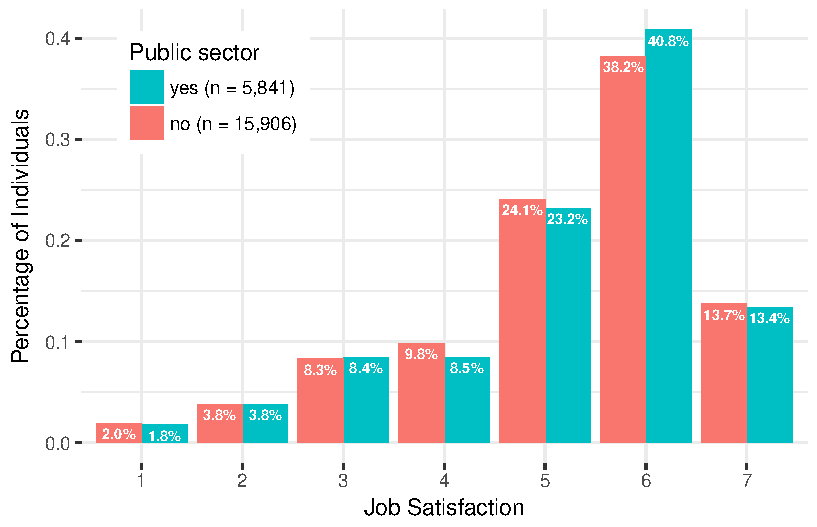
\includegraphics[scale=0.75]{fig.pdf}
\caption{Distribution of job satisfaction anwers between Public and Private Sector Workers} \label{fig:jbsat}
\end{figure} % 2500 words
\chapter{Conclusion}
\label{sec:conclusion}

The purpose of the current study was to evaluate the statistical and practical significance of both the current and the newly proposed fiscal indicators used by the National Treasury Secretariat (NTS) to assess the payment capacity of subnational governments in Brazil. The current methodology enacted in 2012 by the NTS was deemed to be overly complicated in general and also based on a set of fiscal indicators that could potentially be simpler in terms of dimensionality without harm in terms of predictive performance. This view was justified on the basis of the correlation between the fiscal indicators. %add citation

This study has identified that the new methodology that uses only $3$ ratios instead of the $8$ of the current methodology is in fact statistically superior in terms of the likelihood of the given data. This superior performance is mostly attributed to the ratio Current liabilities / Cash and cash equivalents who proved itself to be significant in all specifications employed in this study. 

Expressing these results in the language of the concepts related to fiscal sustainability discussed in section \ref{sec:fiscal-distress}, we can say that empirically, the willingness and ability to pay of an SGN in Brazil appear to be mostly explained by its liquidity position. Solvency ratios appear to be only instrumental for this explanation, in the sense that they matter only to the extent that indirectly they influence the trajectory of liquidity ratios. To exemplify, high debt ratios to net current revenue can only explain fiscal crisis episodes in Brazil to the extent that debt service obligations generate higher current liabilities. 

The research has also shown that for the sample at hand, the fiscal indicators proposed in the new methodology proposed by the NTS could maybe fruitfully include Gross investment in nonfinancial assets / Total expenditure. However, this result appears to be more related to the observed behavior of Rio de Janeiro, who, even in financial difficulties, kept investment rates high because of the commitments made with the 2016 Summer Olympics.

There are four major sources of weakness in this study, all in some way or another related to data constraints. First, we did not allow for the presence of unobservable heterogeneity between states, by using, for example, a fixed effects logit model. The reason for this is simply that in fixed effect estimation all the observations corresponding to states that did not face a crisis episode in the sample horizon would be dropped out of the likelihood function, leaving only the observations of Rio de Janeiro, Rio Grande do Sul and Minas Gerais. 

The second source of weakness is related to the definition of fiscal crisis episode adopted. The enactment of a decree of financial calamity is a political process that a given state might not participate because it does not align with the political calculus of the politicians involved in this decision. Although this sounds like a tautology, it is especially important in the current case. The reason is that the most common interpretation of the Brazilian legal system, shared by the Ministry of Finance\footnote{\url{http://g1.globo.com/bom-dia-brasil/noticia/2016/12/calamidade-financeira-de-estados-nao-e-reconhecida-pelo-governo.html}}, says that the decree of calamity should be restricted to natural disasters, and therefore the benefits, such as the possibility to delay payments to creditors and to bypass some legal requirements for procurement and budgeting process, is not valid under ``financial calamity''. A more reliable definition of fiscal crisis episode would need to make use of arrears data that still do not exist for SGN's in Brazil.

A third source of weakness comes from the 2008-2016 horizon employed. Brazil experienced in the 80s and 90s repeated fiscal crisis of subnational entities with three rounds of debt restructurings. These should clearly be considered a fiscal crisis episode. However, the majority of the explanatory variables used in this study were fiscal variables and indicators derived from the datasets provided by the National Treasury Secretariat. Although, the original period covered by the data published by NTS extends from 1986 through 2016, totalling 31 years of data, events like hyperinflation, change of currencies, change in fiscal reporting and budget classifications and no tracking of stock variables makes the process of compiling a cleaned and consistent dataset a research enterprise of its own.

Finally, because there were only three fiscal crisis episodes in the sample that happened in the same year, it was not possible to look into out of sample forecast accuracy measures, which are ultimately the final yardstick by which EWS models should be judged. \citep{berg2005}.

Putting the need for the collection of a more comprehensive dataset of fiscal variables on SGN aside, the cited weakness of this study are useful alternatives for future work. Additionally, because most of the EWS literature is currently focused on sovereign countries, studies that use different strategies in the three areas that tend to differentiate early warning systems models, namely, the definition of the crisis event, the statistical methodology employed, and the set of explanatory variables, but applied to SGNs, would be a welcome addition to the literature.

 % 1500 words

%-------------------------------------------------------
% POST-TEXT CONTENT


\bibliographystyle{agsm}
{\footnotesize
\bibliography{../references.bib}}

% \appendix
\chapter{Data Definitions and Sources}
\label{appendix:data-source}

The dataset used in this study is available online at 

The majority of the explanatory variables used in this study will be fiscal variables and indicators derived from the datasets provided by the National Treasury Secretariat (STN). This section aim is to address the main data gaps that prevent the use of some specific years in the empirical analysis of this study. The original period covered by the data published by STN extends through 1986 through 2016, totalling 31 years of data. 

The first issue arises in the period from 1980 through 1994 when Brazil was facing a hyperinflation crisis and used several different currencies. Taking into considerations the difficulty in compiling accurate statistics during a period in which prices are changing so rapidly, the possible relevant period is shortened to 1995-2016. 

The second issue is related to the change in fiscal reporting practices brought about by the the Fiscal Responsibility Law in 2000-05-04 and the change in the Economic Classification of expenditures in 2001-05-04. Before this period, only flow variables are published by the STN, and they are not fully consistent with the more recent series. Taking into account the relevance of stock variables for fiscal analysis, the period is again shortened to 2002-2016.

The final issue is related to the conditions surrounding the bailouts provided by the National government. The states were allowed a cap on the maximum amount of debt service that they needed to pay in any given year in terms of their net revenue (Receita Liquida Real), with the difference being incorporated into the debt stock. However, instead of using an accrual basis of accounting, only the interest paid was registered. The central back publishes statistics on an accrual basis for regional governments, but they only begin in 2008. Taking into consideration the relevance of this variable, the period is again shortened to 2008-2016.

\begin{table}[!ht] \centering 
  \caption{Compiled Fiscal Variables} 
  \label{tbl:fares-general} 
{\renewcommand\arraystretch{1.25}}
\begin{tabular} {ccccccc}
\toprule

Report                                 & 
\multicolumn{2}{c}{Fiscal Variable}    & 
\multicolumn{2}{c}{Source}             \\ 

\hline

\multirow{2}{*}{Full}                                          & 
\multicolumn{2}{p{6cm}}{\raggedright full or anytime or open, includes single and return, day single and day return.}                                                 & 
\multicolumn{2}{p{6cm}}{\raggedright Passengers can take any train.}    \\

\hline

\multirow{2}{*}{Reduced}                                                                                     &  
\multicolumn{2}{p{6cm}}{\raggedright reduced or off-peak or saver/super saver, includes single and return, day single and day return for off-peak and supper off-peak.}                                       & 
\multicolumn{2}{p{6cm}}{\raggedright Passengers can take any off-peak train. Peak time may vary from route to route.} \\

\hline

\multirow{2}{*}{Advance}                                                                     & 
\multicolumn{2}{p{6cm}}{\raggedright advance or apex, sold only as single tickets.} & 
\multicolumn{2}{p{6cm}}{\raggedright Passengers can only take the specific train of the ticket. Must be bought in advance and has limited availability}                                                                 \\

\bottomrule
\end{tabular}%
\caption*{Source: Own elaboration}
\end{table} 



\end{document}

